%-----------------------------------------------------------------------
%
\section[Motivation]{Motivation}
Die Positionsbestimmung (Tracking) mittels RFID (Radio-Frequency Identification) bietet gegenüber vergleichbaren Methoden (z.B. Ultraschall, Optisch) verschiedene Vorteile. Das wesentlichste Unterscheidungsmerkmal ist, dass keine direkte Sichtlinie sog. LOS (Line of Sight) notwendig ist um ein Objekt zu lokalisieren. Der Grund dafür ist das zugrunde liegende Messprinzip. Insbesondere im Vergleich mit optischen Verfahren ist RFID damit überlegen. Weiterhin erlauben die als Positionsgeber verwendeten Tags zusätzliche Informationen auf ihnen abzulegen, beispielsweise eine Identifikationsnummer und Weiteres. Dadurch wächst das Anwendungsspektrum weiter. Das Auslesen von zusätzlichen Informationen ist in keiner der anderen Technologien möglich.\\

Das von dem Messsystem der {Amedo GmbH} verwendete Verfahren basiert auf der Messung der Phasenlage der Antwort eines Tags. Die Phasenlage ist direkt proportional zu einer Entfernung. Dabei kommt es aufgrund der Physik im wesentlichen zu folgenden Problemen:
\begin{enumerate}
	\item Die Messung der Position erfolgt über die Auswertung der Phasenlage des empfangenen Signals in Bezug auf ein Referenzsignal. Da in der EU sind nur bestimmte Frequenzen für die Verwendung für RFID erlaubt (865,5–867,5 MHz) kann man die Wellenlänge mit: $ \lambda\simeq0,35 m $ angeben. Daraus folgt, dass alle 35 cm die gleiche Konfiguration der Phase vorliegt. In dieser Arbeit wird dieser Umstand Isophasen genannt. Die gewonnene Information aus der Phase ist somit redundant, d.h. es lässt sich durch die Kenntnis der Phase nicht unmittelbar auf die korrekte Postion schließen. Man kann das Problem umgehen in dem man auf die errechnete Position ein ganzzahliges Vielfaches der Wellenlänge addiert. Die sog. Wellenzahl (vgl.~\eqref{eq:Wavenumbers}).
	\item Das System der Amedo STS verwendet eine spezielle Antennenanordnung um die Position zu ermitteln. Dabei wird eine Antennenanzahl >4 eingesetzt. Für jede dieser Antennen muss eine eigene Wellenzahl bestimmt werden. Durch Auslöschung des Signals, Absorption etc. kann es dazu kommen, dass eine Antenne eine unbestimmte Zeit lang kein Signal vom Tag empfängt. Wenn die Antenne nach dieser Zeit erneut ein Signal empfängt ist die ihr zugehörige Wellenzahl unbekannt und muss neu bestimmt werden. 
	\item In realen Umgebungen treten zusätzlich noch Ruflektionen und ein sog. Multipath-Effekt auf. Dabei wird das Signal nicht auf dem Direkten Weg Antenne-Tag-Antenne empfangen sondern über einen unbekannten, längeren Weg. Dadurch kommt es zu einem Fehler in der Phase. Zusätzlich ist dieser Effekt individuell für jede Antenne.
\end{enumerate}

Eine analytische Lösung des Problems ist schwierig und bisher nicht gelungen. In dieser Arbeit soll mittels numerischer Methoden und Modellen die beschriebenen Probleme zu gelöst werden.

%
%Das Problem liegt in den unbekannten, komplex zu modellierenden Verhalten der elektromagnetischen Funkwellen in geschlossenen Räumen (insb. Auslöschung, Multipath, Reflektion). Diese führen zu einem Fehler der Phase und damit direkt zu einer Falschaussage der Position.\\ \\
%\textbf{Beschreibung der Wellenzahl[Referenz auf die Dipl. Arbeit von Bernd]}\\\\
%Ziel dieser Arbeit ist es ein System zu
%implementieren, das eine direkte Abschätzung (Ad-Hoc-Messung) der Wellenzahl erlaubt.
%Dafür werden Methoden der Numerik verwendet um die Uneindeutigkeit der Phasenlage zu
%eliminieren.
%\\ \\ \\
%Tags gibt es mit unterschiedlichen Funktionsweisen, in dieser Arbeit und in dem von der {Amedo STS} verwendeten System kommen passive Tags zum Einsatz. Diese versorgen sich aus den Funksignalen des Abfragegeräts mit der notwendigen Energie und modulieren ihre "Antwort" auf das Trägersignal auf.\\\\\\
%In der Positionsbestimmung wird im Zusammenhang von "Marker" gesprochen. In der in dieser Arbeit werden RFID-Transponder (sog. Tags) als Marker verwendet. D.h. Es wird die Position im Raum von einem Transponder ermittelt. \\
%

%
%-----------------------------------------------------------------------
%
\section[mathematisches]{Mathematische Voraussetzungen}
%-----------------------------------------------------
Dieser Abschnitt behandelt die mathematischen Voraussetzungen für diese Arbeit.
%
\subsection{Kondition}
%
Gegeben ist ein lineares Gleichungssystem der Form:
$$ \mathbf{A}\mathbf{x}-\mathbf{b} =\mathbf{0} $$
Eine numerische Lösung führt in der Regel zu einer von $\mathbf{0}$ verschiedenen Lösung (insbesondere bei überbestimmten Systemen), so das wir:
$$ \mathbf{A}\mathbf{\tilde{x}}-\mathbf{b} =\mathbf{r} $$
schreiben. Man nennt $\mathbf{r}$ den Residuumvektor. Es ist offensichtlich, dass ein kleines Residuum nicht hinreichend ist um von einem kleinen relativen Fehler auszugehen.\\
Weiter folgt aus $\mathbf{A}\mathbf{x}-\mathbf{b} =\mathbf{0}$ und $\mathbf{A}\mathbf{\tilde{x}}-\mathbf{b} =\mathbf{r}$,dass 
$$ \mathbf{A}\Delta\mathbf{x}=\mathbf{r}$$
und damit:
$ 
\lVert \mathbf{b} \rVert=\lVert \mathbf{Ax} \rVert \leq \lVert \mathbf{A} \rVert \lVert \mathbf{x} \rVert
$, 
$
\lVert \Delta\mathbf{x} \rVert=\lVert -\mathbf{A^{-1}r} \rVert \leq \lVert \mathbf{A^{-1}} \rVert \lVert \mathbf{r} \rVert
$
Wir können nun für den relativen Fehler schreiben:
$$
\frac{\lVert \Delta\mathbf{x} \rVert}{\lVert \mathbf{x} \rVert} \leq 
\frac{\lVert \mathbf{A^{-1}} \rVert \lVert \mathbf{r} \rVert}{\lVert \mathbf{b} \rVert / \lVert \mathbf{A} \rVert} =
\lVert \mathbf{A} \rVert \lVert \mathbf{A^{-1}} \rVert \frac{\lVert \mathbf{r} \rVert}{\lVert \mathbf{b} \rVert}
$$
Der Term $\lVert \mathbf{A} \rVert \lVert \mathbf{A^{-1}} \rVert := \text{cond}(\mathbf{A})$ heißt Konditionszahl. Auch der Begriff Konditionsmaß ist gebräuchlich und bezieht sich auf die gewählte Matrixnorm.
Es kann gezeigt werden, dass $\text{cond}(\mathbf{A}) \gg 1$  für eine schlechte Konditionierung der Matrix steht. Wird im Folgenden von einer speziellen Matrixnorm gesprochen schreiben wir $\text{cond}(\mathbf{A})$ zu 
$$ 
\text{cond}_k(\mathbf{A}) = \lVert \mathbf{A} \rVert_k \lVert \mathbf{A^{-1}} \rVert_k
$$ \\
Der Index $k$ wird entsprechend für die verwendete Norm ersetzt. Beispielsweise ergibt sich für die Konditionszahl der Spektralnorm\footnote{\url{http://de.wikipedia.org/w/index.php?title=Spektralnorm&oldid=118988565}}:
$$ 
\text{cond}_2(\mathbf{A}) = \lVert \mathbf{A} \rVert_2 \lVert \mathbf{A^{-1}} \rVert_2=
\sqrt{\frac{\mu_{max}}{\mu_{min}}}\\
$$
Die Symbole $\mu_{max}$ und $\mu_{min}$ stehen für die Eigenwerte des Systems.\\

Die Konditionszahl ermöglicht eine Analyse der Güte einer Lösung, die mittels Numerischer Verfahren ermittelt wurde. Nach \cite{hermann2006numerische} kann man folgende Aussage über die Konditionszahl treffen:
%
\begin{quote}
"Wird ein lineares Gleichungssystem $Ax=b$ mit $t$-stelliger dezimaler Gleitpunktarithmetik gelöst und beträgt die Konditionszahl $\text{cond}(A) \approx10^\alpha$, so sind auf Grund der im allgemeinen unvermeidbaren Fehler in den Eingabedaten $A$ und $b$ nur $t-\alpha-1$ Dezimalstellen der berechneten Lösung $\tilde{x}$ (bezogen auf die betragsgrößte Komponente) sicher."
\end{quote}

%
\subsection{SVD}
%Um die Konditionszahl zu bestimmen sind aufwändige Berechnungen\footnote{siehe Wochenbericht KW 22} der Eigenwerte der Matrix notwendig. Es wurde nach eine Möglichkeit gesucht diese effizient abzuschätzen oder zu berechnen. Vor Allem soll es auch möglich sein mit dem Verfahren eine nicht symmetrische, nicht quadratische.\\
%Eine Methode die diese Anforderungen erfüllt, ist die sog. Singulärwertzerlegung (im Folgenden SVD := engl. Singular Value Decomposition). 
Bei dem Verfahren der Singular Value Decompostion (oder auch Singulärwertzerlegung), kurz SVD, handelt es sich um eine Faktorisierung einer Matrix. Die Matrix wird dabei als Produkt von drei Matrizen dargestellt. Diese Matrizen enthalten die sog. Singulärwerte und können aus einer der Matrizen abgelesen werden. Die Eigenschaften des Systems sind, ähnlich den Eigenwerten, aus den Singulärwerten bestimmbar. Besonders an der SVD ist, die Existenz für jede Form von Matrix - einschließlich nicht quadratischer Matrizen.\\
Die SVD basiert auf folgender Theorie der linearen Algebra: Jede $M \times N$ Matrix $\mathbf{A}$ kann als Produkt einer $M \times N$ Spalten-orthogonalen Matrix $\mathbf{U}$, einer $N \times N$ Diagonalmatrix $\mathbf{\Sigma}$ mit Werten $\geq 0$ und einer dritten adjungierten $N \times N$-Matrix $\mathbf{V^*}$, so ergibt sich:
%
\begin{equation}
\mathbf{A}= \mathbf{U \Sigma V^*} = \mathbf{U \Sigma V}^T
\end{equation}
Ist $\mathbf{A}$ eine reelwertige Matrix gilt: $ \mathbf{V^*} = \mathbf{V}^T $. Die Matrix $\mathbf{ \Sigma }$ ist im Rahmen dieser Arbeit von besonderem Interesse, denn sie enthält die Singulärwerte $\sigma_r$. Ihre Gestalt ist wie folgt:
%
\begin{equation}
	\mathbf{\Sigma} = \left(\begin{array}{ccc|ccc}
	\sigma_1 &          &          &        & \vdots &        \\
	         & \ddots   &          & \cdots & 0      & \cdots \\
	         &          & \sigma_r &        & \vdots &        \\
	\hline
	         &  \vdots  &          &        & \vdots &        \\
	\cdots   &  0       & \cdots   & \cdots & 0      & \cdots \\
	         &  \vdots  &          &        & \vdots &        \\
	
	\end{array}\right)\nonumber
\end{equation}
%
\phantomeq{\mathbf{\Sigma} = }{ ,wobei~\sigma_1\geq\sigma_2\geq\cdots\geq\sigma_r> 0 \nonumber}
%
Da die $\sigma_r$ der Matrix mit den Eigenwerten in Verbindung stehen, kann aus dieser Matrix die Konditionszahl bestimmt werden. Sie ist durch folgendes Verhältnis gegeben: 
\begin{equation}
	\label{eq:cond_from_svd}
	cond(\mathbf{A})=\frac{max(\sigma_r)}{min(\sigma_r)}=\frac{max(\sigma_1)}{min(\sigma_r)}
\end{equation} 

Es gibt bereits viele Implementationen des Verfahrens, z.B. \cite{press2007numerical}. Diese Implementation wird durch den Erwerb der entsprechenden Lizenz im Rahmen dieser Arbeit verwendet. Weitere Informationen zum Verfahren sind z.B. in \cite[Kaptiel 4.6.3]{bronstejn2012taschenbuch} zu finden.
%
\subsection{Evolutionäre Strategien}
%- Section 1 ----------------------------------------------------------------
\label{seq:EvolutionaryStrategies}
Folgende Information entstammen im Wesentlichen aus \cite{kost2003optimierung},\cite{bronstejn2012taschenbuch}\ sowie \cite{Hansen:1} und sind auf den folgenden Seiten lediglich zusammengefasst und neu arrangiert um eine Einarbeitung in die Thematik zu ermöglichen.\\
%------------------------------------------------------------------
\subsection{Evolutionsstrategien - Grundlagen }
%
Nach dem Vorbild natürlicher Evolution entworfene stochastische Optimierungsverfahren werden Evolutionsstrategie bezeichnet. Sie verwenden die Prinzipien der Mutation, Rekombination und Selektion analog zu der nat. Evolution. Der Grundlegende Ablauf dieser Strategien zeigt die Abbildung~\ref{es_flowchart}\\
Wie in der Natur auch werden Nachkommen aus der Menge der verfügbaren Eltern gebildet. Dabei bezeichnet im Folgenden:
%
\begin{itemize}
	\item $\mu$ die Anzahl der Eltern (=> Größe der Population)
	\item $\lambda$\footnote{Anmerkung: Die Verwendung des Symbols $\lambda$ ist in diesem Kontext nicht eindeutig. Im Rahmen dieser Arbeit steht dieses Symbol auch für die Wellenlänge. In diesem Abschnitt wird jedoch weiterhin $\lambda$ verwendet um die gleiche Nomenklatur wie bei dieser Thematik üblich zu verwenden.} die Anzahl der Eltern die bei Rekombination neue Kinder erzeugt; Die Anzahl der erzeugten Nachkommen einer neuen Generation
	\item $\mathbf{x}_p$ Elternpunkt (Parent)
	\item $\mathbf{x}_c$ Nachkomme einer Generation (Child)
	\item $X_p^1$ Die Menge aller Eltern der ersten Generation $X_p = \{\mathbf{x}_{p_1}^1,..,\mathbf{x}_{p_\mu}^1\}$
	\item $X_p^k$ Die Menge aller Eltern der k-ten Generation $X_p = \{\mathbf{x}_{p_1}^k,..,\mathbf{x}_{p_\mu}^k\}$
\end{itemize}
%
Wir wollen nun in Abbildung~\ref{fig:es_flowchart} einen Blick auf den prinzipiellen Ablauf dieses Algorithmus werfen und anschließend auf die Details eingehen.
%
%------------------------------------------------------------------------------
%------------------------------------------------------------------------------
%------------------------------------------------------------------------------
\begin{figure}[h]
	\begin{center}
		\caption[Ablauf Evolutionsstrategie]{Der Prinzipielle Ablauf des $(\lambda,\mu)$-Evolutionsalgorithmus.}
		\label{fig:es_flowchart}
		\vspace{0.5cm}
		\begin{tikzpicture}[auto]
		\scriptsize
			\tikzstyle{decision} = [diamond, draw=black, thick, fill=black!20, text width=5em, text badly centered, inner sep=1pt]
%			
			\tikzstyle{block} = [rectangle, draw=black, thick, fill=gray!20, text width=15em, text centered, rounded corners, minimum height=4em]
%	
			\tikzstyle{line} = [draw, thick, -latex',shorten >=1pt];
			\tikzstyle{commentline} = [draw, dashed, green!50,-latex',shorten >=1pt];
%	
			\tikzstyle{cloud} = [ dotted, draw=green!50, thick, ellipse,,fill=green!20, minimum height=2em, text width= 10em, text badly centered];
%	
			\matrix [column sep=5mm,row sep=7mm]
			{
				% row 1
				& \node [block] (start) { Start }; & \\
				% row 2
				&\node [block] (init) {Erstelle Startpopulation $X_p^1$ bestehend aus $\mu$-Individuen }; & 
				\node [cloud] (comment1) {Initialisierung, mit Zufallswerten}; \\
				% row 4
				& \node [block] (identify) {Erzeuge eine Menge von $\lambda$ Nachkommen $X_c^k$ aus der aktuellen Elterngeneration $X_p^k$ durch Rekombination \&\&, || Mutation}; & \\
				% row 5
				\node [block] (update) {Nächste Stufe der Evolution; k++}; &
				\node [block] (evaluate) {Durch Selektion die besten $\mu$ Nachkommen für die Generation $X_p^{k+1}$ auswählen}; & \\
				% row 6
				& \node [decision] (decide) {$\Delta \geq \Delta_{min}$}; & 
				\node [cloud] (criteria) {Abbruchkriterium; Muss geeignet gewählt werden, bspw. max. Anzahl der Generationen oder Erreichen des Optimums};\\
				% row 7
				& \node [block] (stop) {Ende}; & \\
			};
% Arrows
			\tikzstyle{every path}=[line]
			\path (init) -- (identify);
			\path (identify) -- (evaluate);
			\path (evaluate) -- (decide);
			\path (update) |- (identify);
			\path (decide) -| node [near start] {Ja} (update);
			\path (decide) -- node [midway] {Nein} (stop);
			\path (start) -- (init);
			
			\tikzstyle{every path}=[commentline]
			\path (criteria) -- (decide);
			\path (comment1) -- (init);
			
		\end{tikzpicture}
	\end{center}
\end{figure}
%------------------------------------------------------------------
\subsubsection[Mutation]{Mutation}
Ein Nachkomme $\mathbf{x}_C$ wird aus seinem Elternteil $\mathbf{x}_P$ und einer zufälligen Variation $\mathbf{d}$ gebildet.
\begin{equation} \label{eq:Mutation_Child}
	\mathbf{x}_c = \mathbf{x}_P + \mathbf{d}
\end{equation}
Dabei ist $\mathbf{d}$ ein bei jeder Mutation neu zu bestimmender $(0,\sigma^2)-normalverteilte$ Zufallszahl $Z(0,\sigma^2)$:
\begin{equation}\label{eq:wavenumber_trilateration_model2}
\mathbf{d}=
\left(
	\begin{array}{c}
		d_1 \\
		\vdots\\
		d_n 
	\end{array}
\right)
=
\left(
	\begin{array}{c}
		Z(0,\sigma_1^2) \\
		\vdots\\
		Z(0,\sigma_n^2) 
	\end{array}
\right)
=
\left(
	\begin{array}{c}
		Z(0,1) \sigma_1 \\
		\vdots\\
		Z(0,1) \sigma_n 
	\end{array}
\right)
\end{equation}
%
Die Normalverteilung der Variation ist nützlich, da kleine Änderungen wahrscheinlicher sind als große. Die maximale Größe der Variation wird durch die Standardabweichung $\sigma_i$ bestimmt. Sie steuert somit die Schrittweite von Generation zu Generation.
%
%------------------------------------------------------------------
\subsubsection[Rekombination]{Rekombination}
Durch Rekombination zweier oder mehr Eltern aus der Menge aller $\mu$-Eltern $X_{\varrho} \subset X_E$. Die Wahl der Eltern sollte zufällig erfolgen um Inzuchtprobleme zu verhindern.\\
Zwei Arten der Rekombination sind denkbar:\\

Die \textit{intermediär Rekombination} erstellt einen Nachkommen durch das gewichtete Mittel von $\varrho$ Eltern.
%
\begin{equation}
\mathbf{x}_c = \Sigma^\varrho_{i=1} \alpha_i\mathbf{x}_{p_i},\\ \Sigma^\varrho_{i=1} \alpha_i = 1,\\ 2\leq\varrho\leq\mu
\end{equation} 
%
Bei der \textit{diskreten Rekombination} vom $\varrho$-Eltern wird die \textit{i}-te Komponente $x_{ic}$ eines Nachkommen $\mathbf{x}_c$ mit der \textit{i}-te Komponente eines zufällig gewählten Elternpunktes gleichgesetzt.
%
\begin{equation}
\mathbf{x}_{ic} = \mathbf{x}_{ip_j},\\ j\in\{1,...,\varrho\},\\i=1,...,n
\end{equation} 
%
%- Section .4 -----------------------------------------------------------------
\subsubsection[Selektion]{Selektion}
Die durch Rekombination und/oder Mutation erzeugten Nachkommen werden in dem Schritt Ausgewählt um einen Evolutionsfortschritt zu erreichen. Dies erfolgt anhand des Vergleichs mit dem Zielfunktionswert $f(\mathbf{x})$. Das beste Individuum oder die besten werden für die nachfolgende Generation ausgewählt. Dabei gibt es Strategien bei denen nur die Nachkommen an der Auswahl beteiligt sind und welche bei denen Eltern und Kinder teilnehmen.

%- Section .5 -----------------------------------------------------------------
\subsubsection{Evolutionsalgorithmus}
%
Der eigentliche Evolutionsalgorithmus ist in Abbildung~\ref{fig:es_flowchart} dargestellt. Er enthält im wesentlichen die in den vorherigen Abschnitten beschriebenen Schritte. Der prinzipielle Ablauf ist für alle Evolutionsalgorithmen gleich. Eine Unterscheidung der Verfahren kann durch verschiedene Parameter beschrieben werden. Wesentlich dabei sind die Populationsgröße $\mu$, die Anzahl an der Rekombination beteiligten Eltern $\varrho$, die gewählte Selektionsstrategie sowie die Anzahl der Nachkommen $\lambda$. Im Folgenden sind zuerst einige Beispiele für die Nomenklatur der Selektionsstrategie aufgeführt, die im Anschluss genauer beschrieben werden.\\
Für Strategien die nur auf Mutation für die Erzeugung von Nachkommen setzten sind folgende Nomenklaturen gebräuchlich:
\begin{itemize}
\item $(\mu+\lambda)$ Elternelemente werden in der Selektion berücksichtigt
\item $(\mu,\lambda)$ Ausschließlich Nachkommen nehmen an der Selektion teil
\end{itemize}
%
Die Strategien werden Plus- bzw. Komma-Strategie genannt. bei der Plus-Strategie wird zusätzlich noch ein gewichtungsfaktor eingeführt, der das "altern" der Elterngeneration darstellt. Dieser Mechanismus soll verhindern, dass die Eltern, nach einer gewissen Anzahl an Generationen, nicht mehr berücksichtigt werden.\\
Wird die Rekombination eingesetzt kann auch die Anzahl der beteiligten Elternelemente angegeben werden:
\begin{itemize}
\item $({\mu}/{\varrho}+\lambda)$ \& $({\mu}/{\varrho},\lambda)$ Angabe der Anzahl beteiligter Eltern bei der Rekombination.
\end{itemize}
%
Mithilfe der hier beschrieben Klassifikationen werden die Algorithmen im Folgenden stets angegeben.\\

In Abbildung~\ref{fig:es_flowchart} wird der Ablauf einer Optimierung mit evolutionären Verfahren dargestellt. Es wird die Komma-Strategie gezeigt, ein Struktogramm der Plus-, oder anderer Strategien ist nicht gezeigt. Die Unterschiede würden sich in dem Punkt Rekombination zeigen.
%
%------------------------------------------------------------------------------
%- Section .6 -----------------------------------------------------------------
\subsection{Strategien mit mehreren Populationen}
Es ist möglich die Strategien auf die Ebene von Populationen zu erweitern. Das bedeutet, man lässt ganze Populationen miteinander in Wettstreit treten und nur diejenige überleben, die die besten Ergebnisse liefern. Das mündet in einem zweistufigen Evolutionsprozess. Man kann die Notation um diesen Umstand erweitern und erhält so:
$$
[\mu_2/\varrho_2,^{+}\lambda_2(\mu_1/\varrho_1,^{+}\lambda_1)]
$$
Sprich aus $\mu_2$-Elternpopulationen werden durch Rekombination mit jeweils $\varrho_2$ Populationen, $\lambda_2$ Nachkommenpopulationen generiert. Innerhalb der Populationen erfolgt die Optimierung anhand einer $({\mu_1}/{\varrho_1}+\lambda_1)$ oder $({\mu_1}/{\varrho_1},\lambda_1)$-Strategie. Nun kann nach einer bestimmten Zahl von Generationen die besten Populationen für die nächste Generation ausgewählt werden. Auch hier stehen verschiedene Auswahlkriterien zur Verfügung. Man kann z.B. die Population anhand des Zielfunktionswert des besten Individuums wählen oder den Mittelwert über alle Individuen wählen.
%
%- Section .7 -----------------------------------------------------------------
\subsection{Optimierungsräume}
\lipsum[1]
%
\subsubsection{Kontinuierliche Optimierung}
%
\lipsum[1]
%
\subsubsection{Diskrete Optimierung}
%
\lipsum[1]
%
\subsubsection{Gemischte Optimierung}
%
\lipsum[1]
%
%- Section .8 -----------------------------------------------------------------


%
\subsection{Phase und Wellenzahl}
\begin{figure} [h]
\centering
         \caption[Zusammenhang Wellenlänge - Wellenzahl]{Dargestellt ist der Zusammenhang zwischen der Wellenlänge $\lambda$ und der Wellenzahl $n$. Da die Phase alle $2\pi$ den gleichen Wert annimmt, wird mit dem Faktor $n$ ein vielfaches der Wellenlänge aufaddiert. Dadurch erhält man die Entfernung zu dem Tag.}
         \label{fig:wavenumber_wavelength}
         \vspace{0.5cm}
         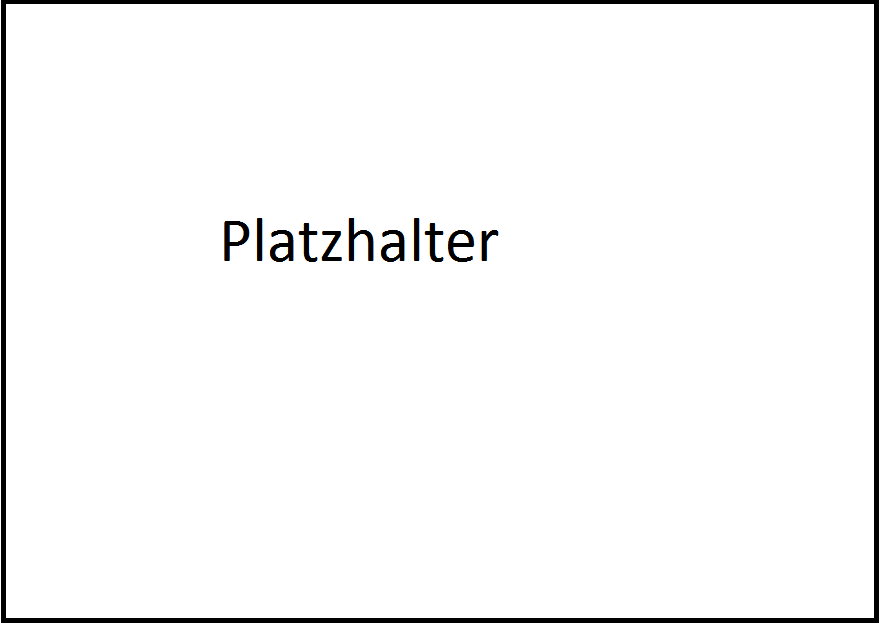
\includegraphics[width=\textwidth]{img/00_placeholder.png}
%      
\end{figure}

Aus der Abbildung~\ref{fig:wavenumber_wavelength} lässt sich folgender Zusammenhang ableiten.
%
\begin{equation}
\label{eq:Phase_Wavenumber}
	d(\Theta, n)=\lambda(\Theta+n)
\end{equation}

\lipsum[1]

%
%
%-----------------------------------------------------------------------
%
\section[technisches]{Technische Voraussetzungen}
%-----------------------------------------------------
In diesem Abschnitt werden die technischen und physikalischen Grundlagen für diese Arbeit vorgestellt und das Wichtigste erörtert. Es wird auf die Besonderheiten und Merkmale des auf Funk basierenden RFID-Verfahrens eingegangen. Die andere Trackingverfahren werden, aufgrund der Unterschiedlichkeit der Systeme wird im Rahmen dieser Arbeit nicht weiter behandelt. Es kann nicht im vollem Umfang auf die Details der Technik eingegangen werden ohne den Rahmen dieser Arbeit zu sprengen. Interessierte sei die referenzierte Literatur für eine weite Lektüre empfohlen.\\
%
%
\subsection{Positionsgenauigkeit auf Funk basierender Verfahren}
\label{sec:RFID_Accuracy}
Die Positionsgenauigkeit eines auf EM basierenden Systems ist von dem Messprinzip abhängig. Dabei bieten sich im Wesentlichen drei Möglichkeiten:\\
%
\begin{table} [ht!]
	\begin{center}
		\begin{tabular}{lp{65mm}p{15mm}}
		1. & Laufzeitmessiung & \textbf{TOA} \\
		2. & Messung der Signalsträrke & \textbf{RSSI} \\
		3. & Phasendifferenzmessung & \textbf{PD} \\
		\end{tabular}
	\end{center}
\end{table}
%
Eine Laufzeitmessung des Signals kommt aufgrund der Ausbreitungsgeschwindigkeit der EM-Welle nicht in Frage, da diese typischerweise gleich der Lichtgeschwindigkeit ist und die Distanz zwischen Sender und Empfänger zu gering ist. Das reduziert die Möglichkeiten auf zwei Verfahren.
Bei der RSSI wird die Stärke des empfangenen Signals ausgewertet. Dies stellt eine einfache Art der Positionsermittelung dar. Jedoch kann die Signalstärke stark schwanken und erlaubt nur eine geringe Ortsauflösung.
Bei der PD wird die Postion anhand der zurückgestrahlten Welle ermittelt, genauer der Phase der Welle.

\subsection{RFID}
%
Bei \textit{Radio-Frequency Identification} (RFID) handelt es sich um einen Funkstandard der die kontaktlose Identifikation bei gleichzeitiger Erfassung zusätzlicher Informationen ermöglicht (Payload). Zur Technik gehört ein Auslesegerät (Reader) und ein oder mehrere Transponder (Tags). Eine sehr grobe Übersicht über typische Bauformen von Tags und Reader ist in \ref{fig:RFID_TAGS_AND_READER} zu finden. Die dargestellten Tags sind für verschiedene Frequenzbänder. Heute verfügbare Transponder lasen sich auf nahezu jeder beliebigen Oberfläche anbringen. Das ermöglicht ein großes Anwendungsspekrum, praktisch wird die Technik in jeder Umgebung eingesetzt in der es erforderlich oder nützlich ist, Dinge kontaktlos zu identifizieren. Eine gute Übersicht über Branchen und Anwendungsgebiete für RFID ist in \cite{RFIDJournal} zu finden. Im Rahmen dieser Arbeit wird kein umfassender Überblick über die Technik geboten, da die Bauformen und Spezifikationen sehr stark variieren. Ein Umfassendes Werk, gute Einführung und Übersicht zur Technik bietet~\cite{finkenzeller2008rfid}. Dort werden auch detailliert die physikalischen Grundlagen verschiedener Antennenbauformen und Tags erläutert. Aufgrund des großen Anwendungsspektrums und der weiten Verbreitung ist die Technik in die Kritik geraten. Unter dem Dach des Vereins \textit{digitalcourage e.V.} existiert die Kampange \textit{StopRFID}. Die Kampagne hat sich zum Thema gemacht über die Anwendungsmöglichkeiten und Risiken von RFID aufzuklären \cite{stoprfid2013}. Die Seiten der Kampagne bieten eine sehr weitgehende Auflistung der Anwendungen für RFID.\\
%Ziel der Kampagne ist es die Gefahren in den gesellschaftlichen Fokus zu rücken und für den Umgang mit der allgegenwärtigen Technik zu sensibilisieren. Die Kampagne über sich selbst:
%\begin{quote}
%"Wir wollen RFID nicht komplett verhindern. Es geht uns nicht darum, die RFID-Entwicklung zum Erliegen zu bringen ... Im Gegenteil." \footnote{\url{http://www.foebud.org/rfid/was-kann-ich-tun/}}
%\end{quote}
%
\begin{figure} [h!]
\centering
         \caption[Beispiele für Transponder und Lesegeräte]{ Hier gezeigt sind Beispiele für RFID Transponder und Lesegeräte. Das linke Bild zeigt drei typische Tags, nahezu jede Gestalt ist mittlerweile erhältlich. Die hier gezeigten Tags eignen sich für eine Anbringung an glatten Oberflächen. Es gibt zig weitere Bauformen, die unterschiedlichste Anwendungsspektren bedienen und sogar eine Implantation ermöglichen (nicht gezeigt). Im rechten Bild ist ein Handlesegerät gezeigt. Zum Mobilen Auslesen über mittlere bis kurze Distanzen. Auch bei den Readern gibt es unterschiedlichste Bauformen, die je nach Anwendungsfall ausgewählt werden.}
         \label{fig:RFID_TAGS_AND_READER}
         \vspace{0.5cm}%         
         \begin{subfigure}[h]{0.4\textwidth}
                 \centering
                 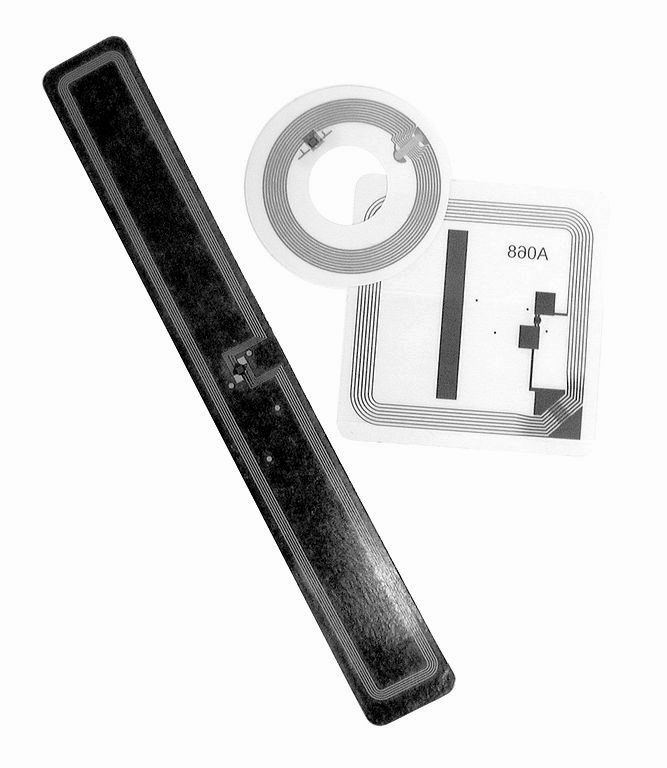
\includegraphics[width=\textwidth]{img/667px-RFID_Tags_gs.png}
                 \vspace{.1cm}
                 \caption{ RFID- Transponder}
                 \label{fig:TAGS}
         \end{subfigure}
%         
\qquad
%
         \begin{subfigure}[h]{0.4\textwidth}
                 \centering
                 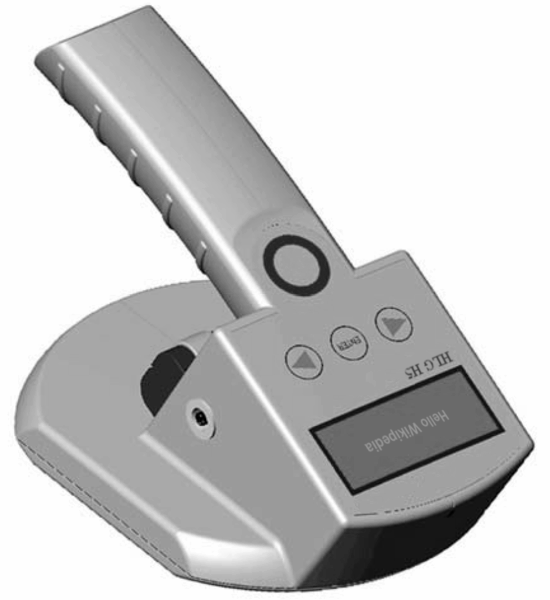
\includegraphics[width=\textwidth]{img/RFID-Reader_gs.png}
                 \vspace{.1cm}
                 \caption{RFID- Handlesegerät }
                 \label{fig:READER}
         \end{subfigure}
\end{figure}
%
\label{sec:Measurement1}
%
%

Die Messung der Position erfolgt über die Auswertung der Phasenlage des empfangenen Signals in Bezug auf ein Referenzsignal. In der EU gibt es verschiedene zulässige RFID-Frequenzen sie reichen von $865,0$ MHz bis $868,0$ MHz~\cite{etsi1}. Man kann man die Wellenlänge mit: $ \lambda\simeq0,35 m $ angeben. Daraus folgt, dass alle 35 cm die gleiche Konfiguration der Phase vorliegt. Im Rahmen dieser Arbeit wird dabei von \textit{Isophasen} gesprochen. Daraus folgt, dass die gewonnene Information aus der Phase ist nicht eindeutig ist. D.h. es lässt sich durch die Kenntnis der Phase nicht unmittelbar auf die korrekte Postion des Tags schließen. Man kann das Problem umgehen in dem man auf die errechnete Position ein ganzzahliges Vielfaches der Wellenlänge addiert, siehe Gleichung~\ref{eq:Phase_Wavenumber}. Die dort beschriebene Konstante $n$ wird Wellenzahl genannt.\\
%

Das System der Amedo STS verwendet eine spezielle Antennenanordnung um die Position zu ermitteln. Dabei wird eine Antennenanzahl >4 eingesetzt. Für jede dieser Antennen muss eine eigene Wellenzahl bestimmt werden. Durch Auslöschung des Signals, Absorption etc. kann es dazu kommen, dass eine Antenne eine unbestimmte Zeit lang kein Signal vom Tag empfängt. Wenn die Antenne nach dieser Zeit erneut ein Signal empfängt ist die ihr zugehörige Wellenzahl unbekannt und muss neu bestimmt werden. \\
%

In realen Umgebungen treten zusätzlich noch Reflektionen und ein sog. Multipath-Effekt auf. Dabei wird das Signal nicht auf dem Direkten Weg Antenne-Tag-Antenne empfangen sondern über einen unbekannten, längeren Weg. Dadurch kommt es zu einem Fehler in der Phase. Zusätzlich ist dieser Effekt individuell für jede Antenne.
%

\subsection{PRPS-Messystem}
%
\begin{floatingfigure}[hr!]{7cm}
         \centering
         \caption[PRPS der \amedogmbh]{Abgebildet ist der Messaufbau aus vier Antennen. In dem Aufbau verbaut sind die wesentlichen elektronischen Komponenten wie Auswerte- und Steuereinheit. Nicht einzeln gezeigt.}
         \vspace{2mm}
         \label{fig:System}
         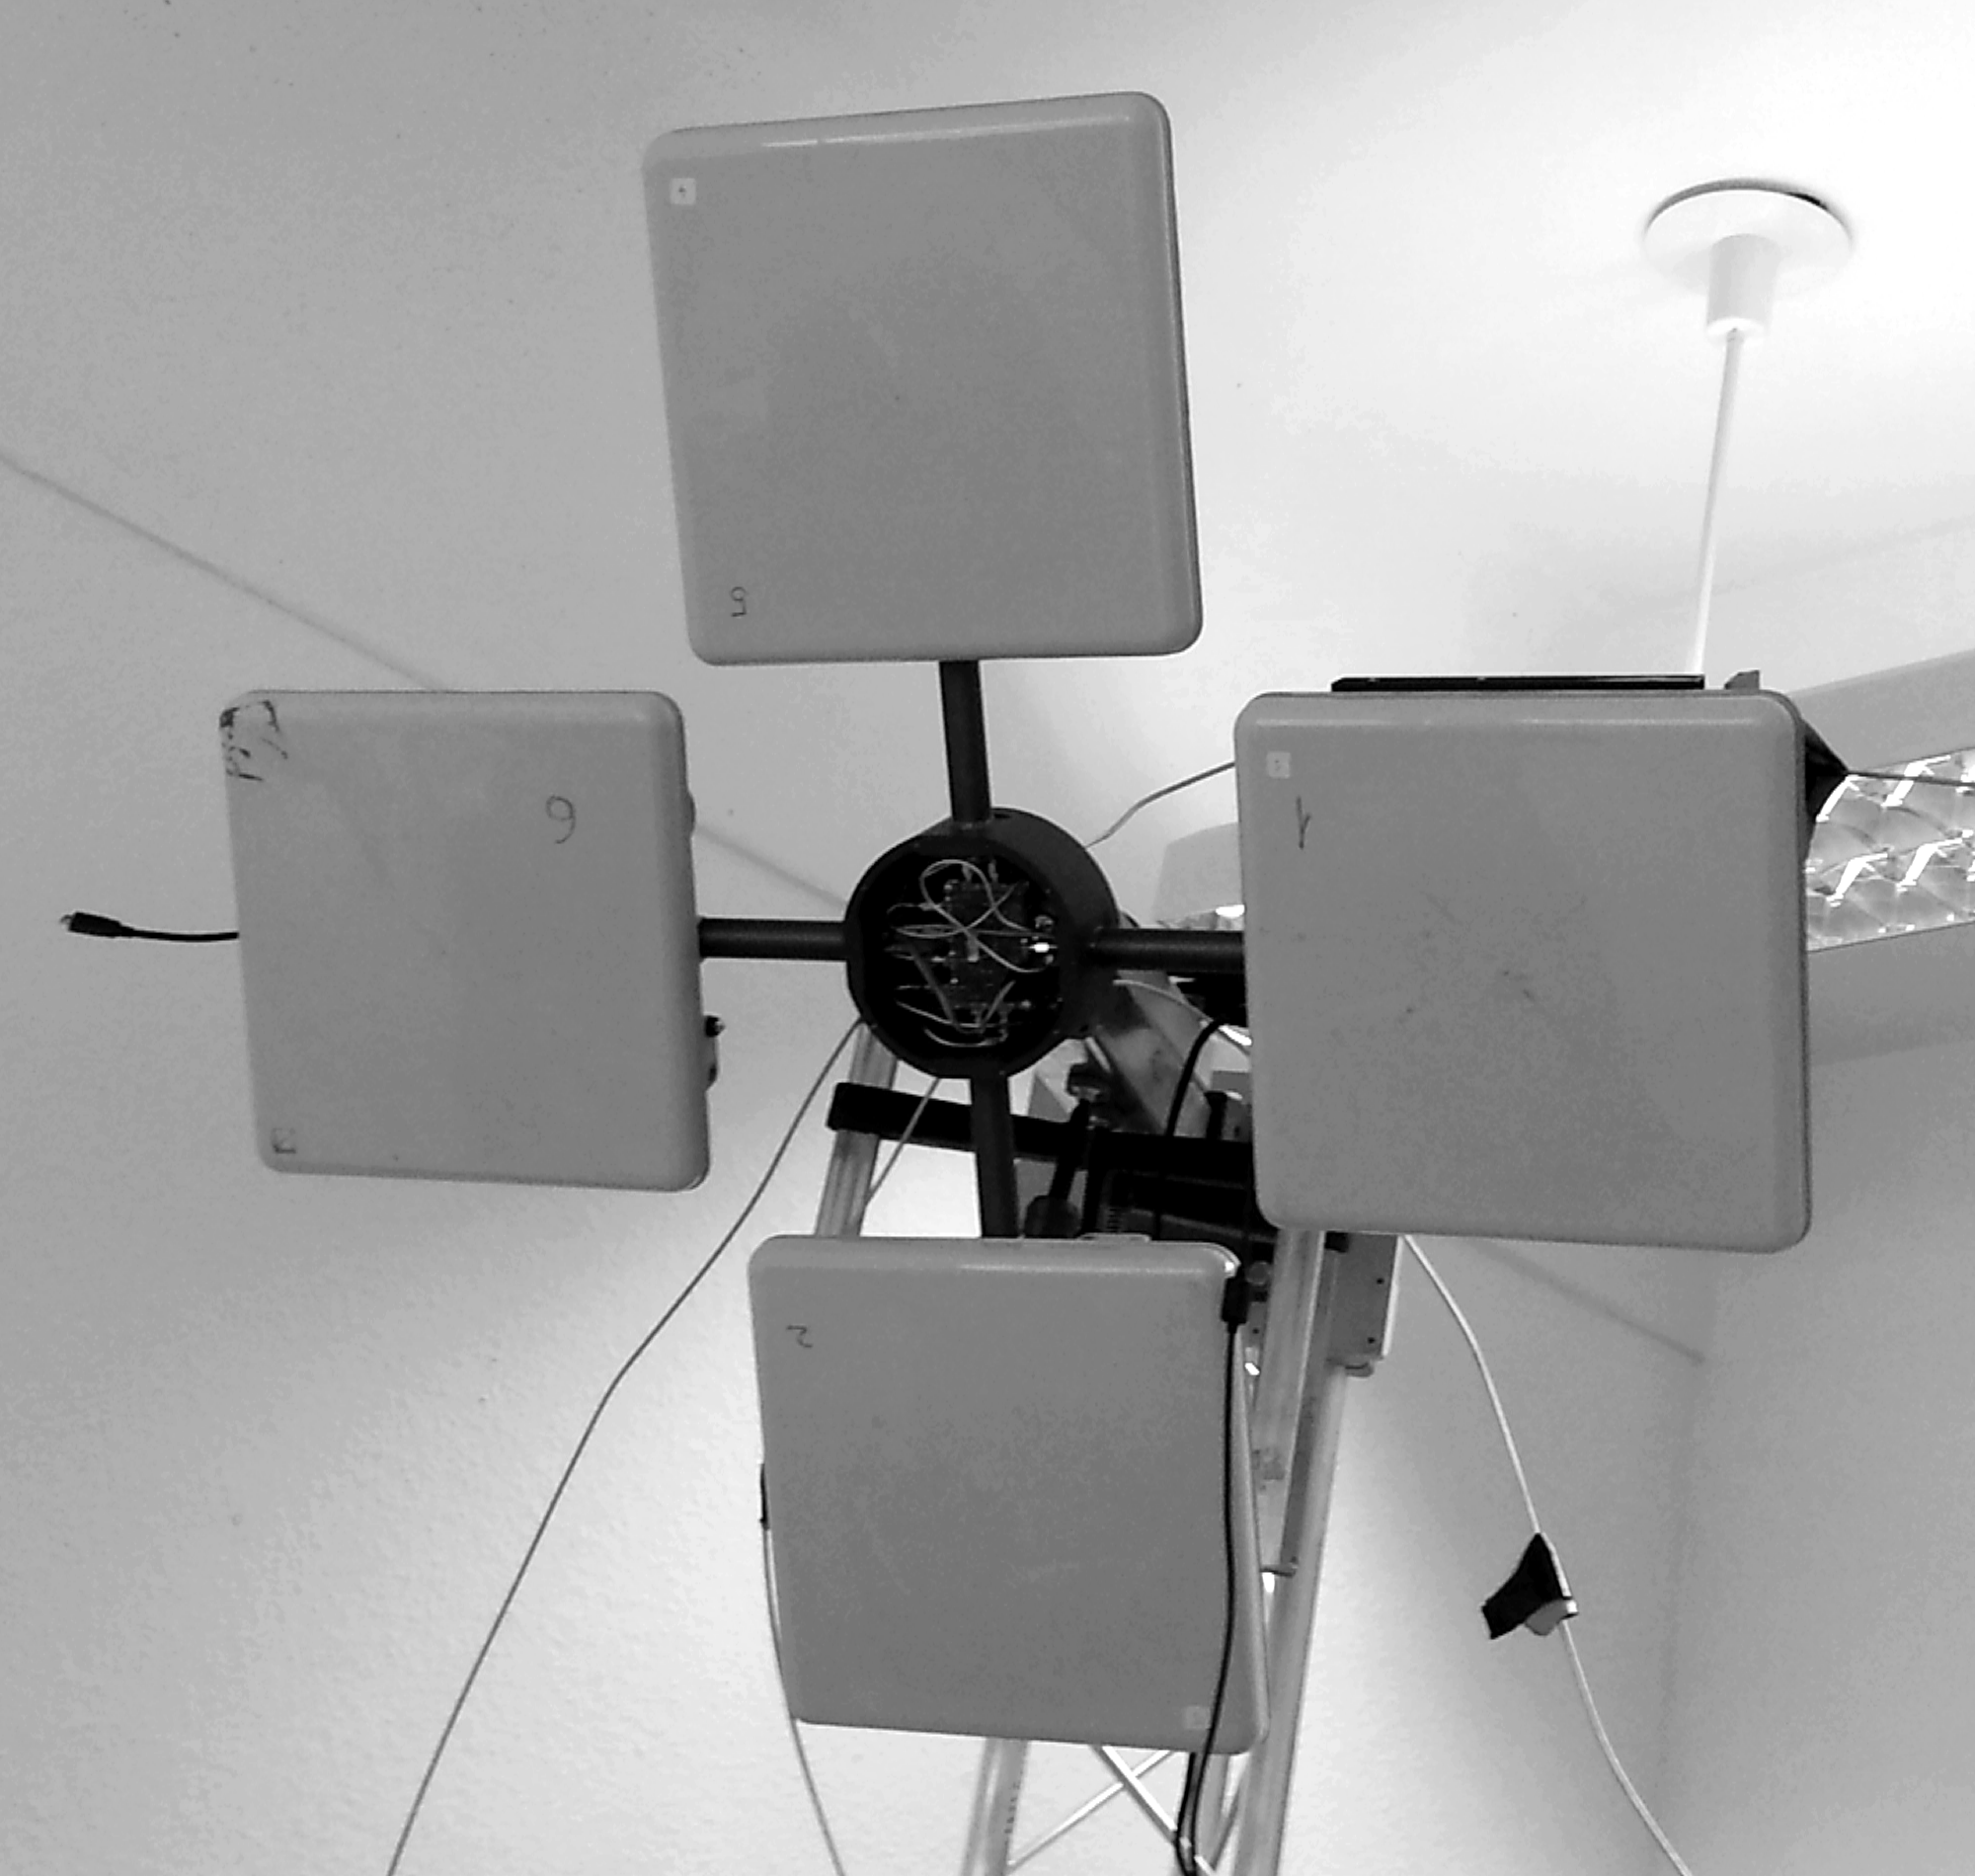
\includegraphics[width=0.4\textwidth]{img/4AntennaSetup_small.png}
         \vspace{2mm}
%         
\end{floatingfigure}
%
Diese Arbeit wird für das Messsystem der \amedogmbh entwickelt. Die Entwicklung wird Teil der Softwarekomponenten des Systems werden. Aktuelle befindet sich das gesamte System in der Revision, in diesem Abschnitt wird der Stand der Entwicklung dargestellt. Details über Hardware und Software werden im Rahmen der Arbeit nicht besprochen, sofern sie diese Arbeit nicht unmittelbar betreffen. \\
%

Das auf RFID basierende PRPS (Passiv RFID Positioning System) besteht aus mehreren frei positionierbaren Antennen. Eine Mess- und Steuereinheit sowie einem Rechner zur Kommunikation mit Endkundensoftware. Die Systemkomponenten für die Messwertaufnahme und Steuerung sind in einem Gehäuse untergebracht, dieses zeigt Abbildung~\ref{fig:System}. Eine typische Installation ist in Abbildung~\ref{fig:Setup} gezeigt. Dort wurde ein System mit insgesamt acht Antennen installiert. Vier Antennen sind frei aufgestellt, vier Weitere in einer festen Anordnung (\textit{Spinne}) installiert. Der Aufbau ist auf ein Messvolumina gerichtet.\\
%
\subsubsection{Leistungsmerkmale}
%
Das PRPS erlaubt eine Identifikation mehrerer Objekte oder genauer: RFID-Tags die auf den Objekten angebracht sind. Wird ein einzelner Tag ausgewählt kann seine Postion mit einer einer sehr hohen Frequenz ausgegeben werden. Die momentan Erreichbare Werte liegen bei $60$~Hz. Je nach Umgebung kann dieser Wert jedoch Variieren, siehe Kapitel~\ref{sec:Komplexity1}. Sollen mehrere Tags ausgegeben werden, verringert sich die Frequenz entsprechend. Bei der Verwendung von drei Tags ist einer Leserate von $20$~Hz pro Tag realistisch. Die Positionsgenauigkeit liegt aktuell bei $\approxeq 5$~mm. Die Antennen können frei Arrangiert werden. Das erlaubt eine Anpassung an nahezu jeden Raum und jeden Kundenbedarf. Als Tags kommen jeder Handelsübliche RFID-Tag im verwendeten Frequenzband im Bereicht der ETSI-Frequenzen~\cite{etsi1} in Frage. Der Messbereich liegt bei mehreren Kubikmetern und einer erprobten maximalen Entfernung von $6-7$~Metern. Theoretisch ist das maximale Volumen noch größer. Die leistungstarke Messeinheit besteht aus einer sehr flexiblen Messelektronik. Diese ist in der Lage eine sehr hohe Güte und Frequenz der Messwerte zu realisieren.\\

%
\begin{figure}[h]
         \centering
         \caption[Messaufbau der Amedo GmbH]{Abgebildet ist der Messaufbau mit unterschiedlichen Antennen. Der Aufbau ist auf ein Messvolumina von mehreren Kubikmetern ausgerichtet}
		\label{fig:Setup}
		\vspace{2mm}
         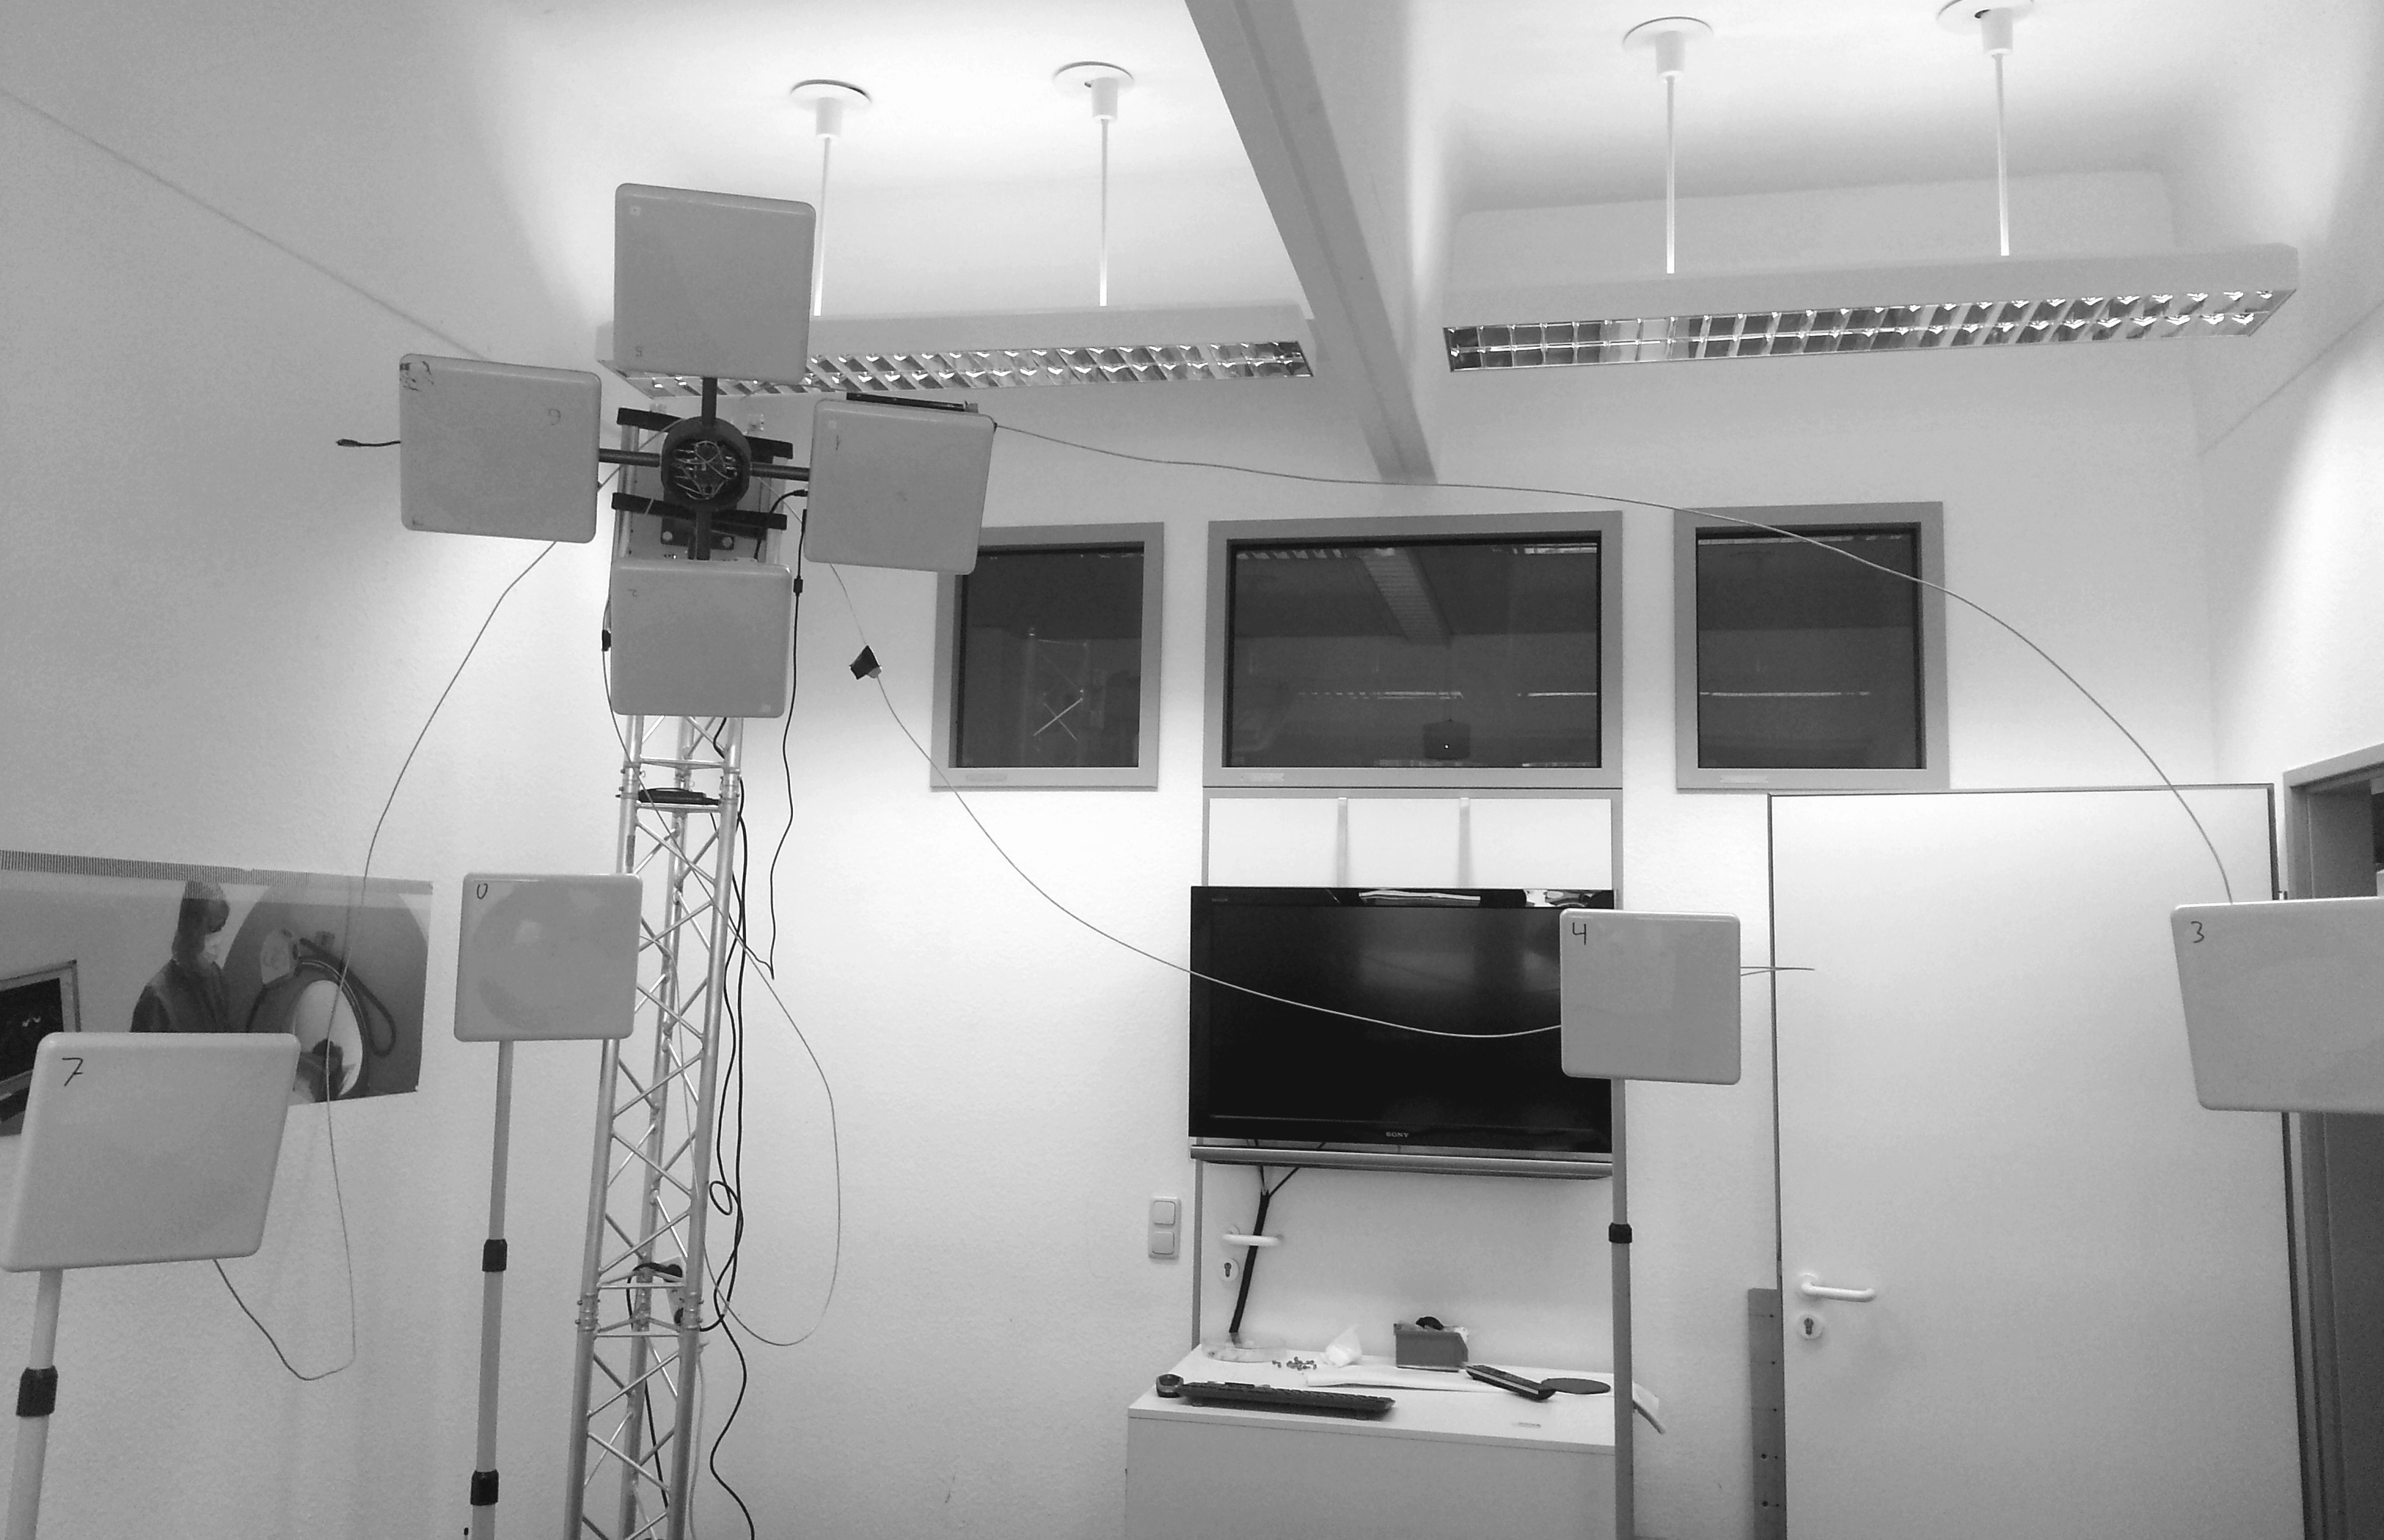
\includegraphics[width=\textwidth]{img/RFID-Okto.png}
         
\end{figure}
%
%-----------------------------------------------------------------------
\section{Anforderungen an die Lösung}
Aus den bisher vorgestellten Überlegungen können nun folgende Anforderungen abgeleitet werden:
%
\begin{enumerate}
	\item Lösung muss schnell (ideal < 1 Sekunde) gefunden werden
	\item Unabhängigkeit von Stütz- Kalibrierpunkten
	\item Eindeutigkeit der Lösung
	\item Eignung für ein großes Messvolumen
	\item Nahtlose Integration in das bestehende Software Ökosystem
%
\end{enumerate}
%
\section{Ziel und Herangehensweise}
%
Das Ziel der Arbeit ist die Entwicklung eines Systems zur Ermittelung der Wellenzahl. Gleichzeitig sollen die oben abgeleiteten Anforderungen erfüllt werden. Das System wird im Kern die Lösung über numerische Verfahren finden, im speziellen kommt das sog CMA-ES zum Einsatz. Dazu wird zuerst ein Modell entworfen werden, dass sich für dieses Verfahren eignet. Das Modell soll mit möglichst wenig Annahmen/ Einschränkungen auskommen und dennoch ein relativ sicheres, reproduzierbares Ergebnis liefern. Das System soll unmittelbar in den Produkten der \amedogmbh zum Einsatz kommen können. Darüber hinaus soll im Rahmen dieser Arbeit eine Methode entwickelt werden, um die Position von frei im Raum angeordnete Antennen zu ermitteln.
%
%-----------------------------------------------------------------------
